\documentclass{standalone}
\usepackage{tikz}
\usetikzlibrary{patterns, positioning}
\usepackage[sfdefault]{ClearSans} %% option 'sfdefault' activates Clear Sans as the default text font
\usepackage[T1]{fontenc}

\begin{document}
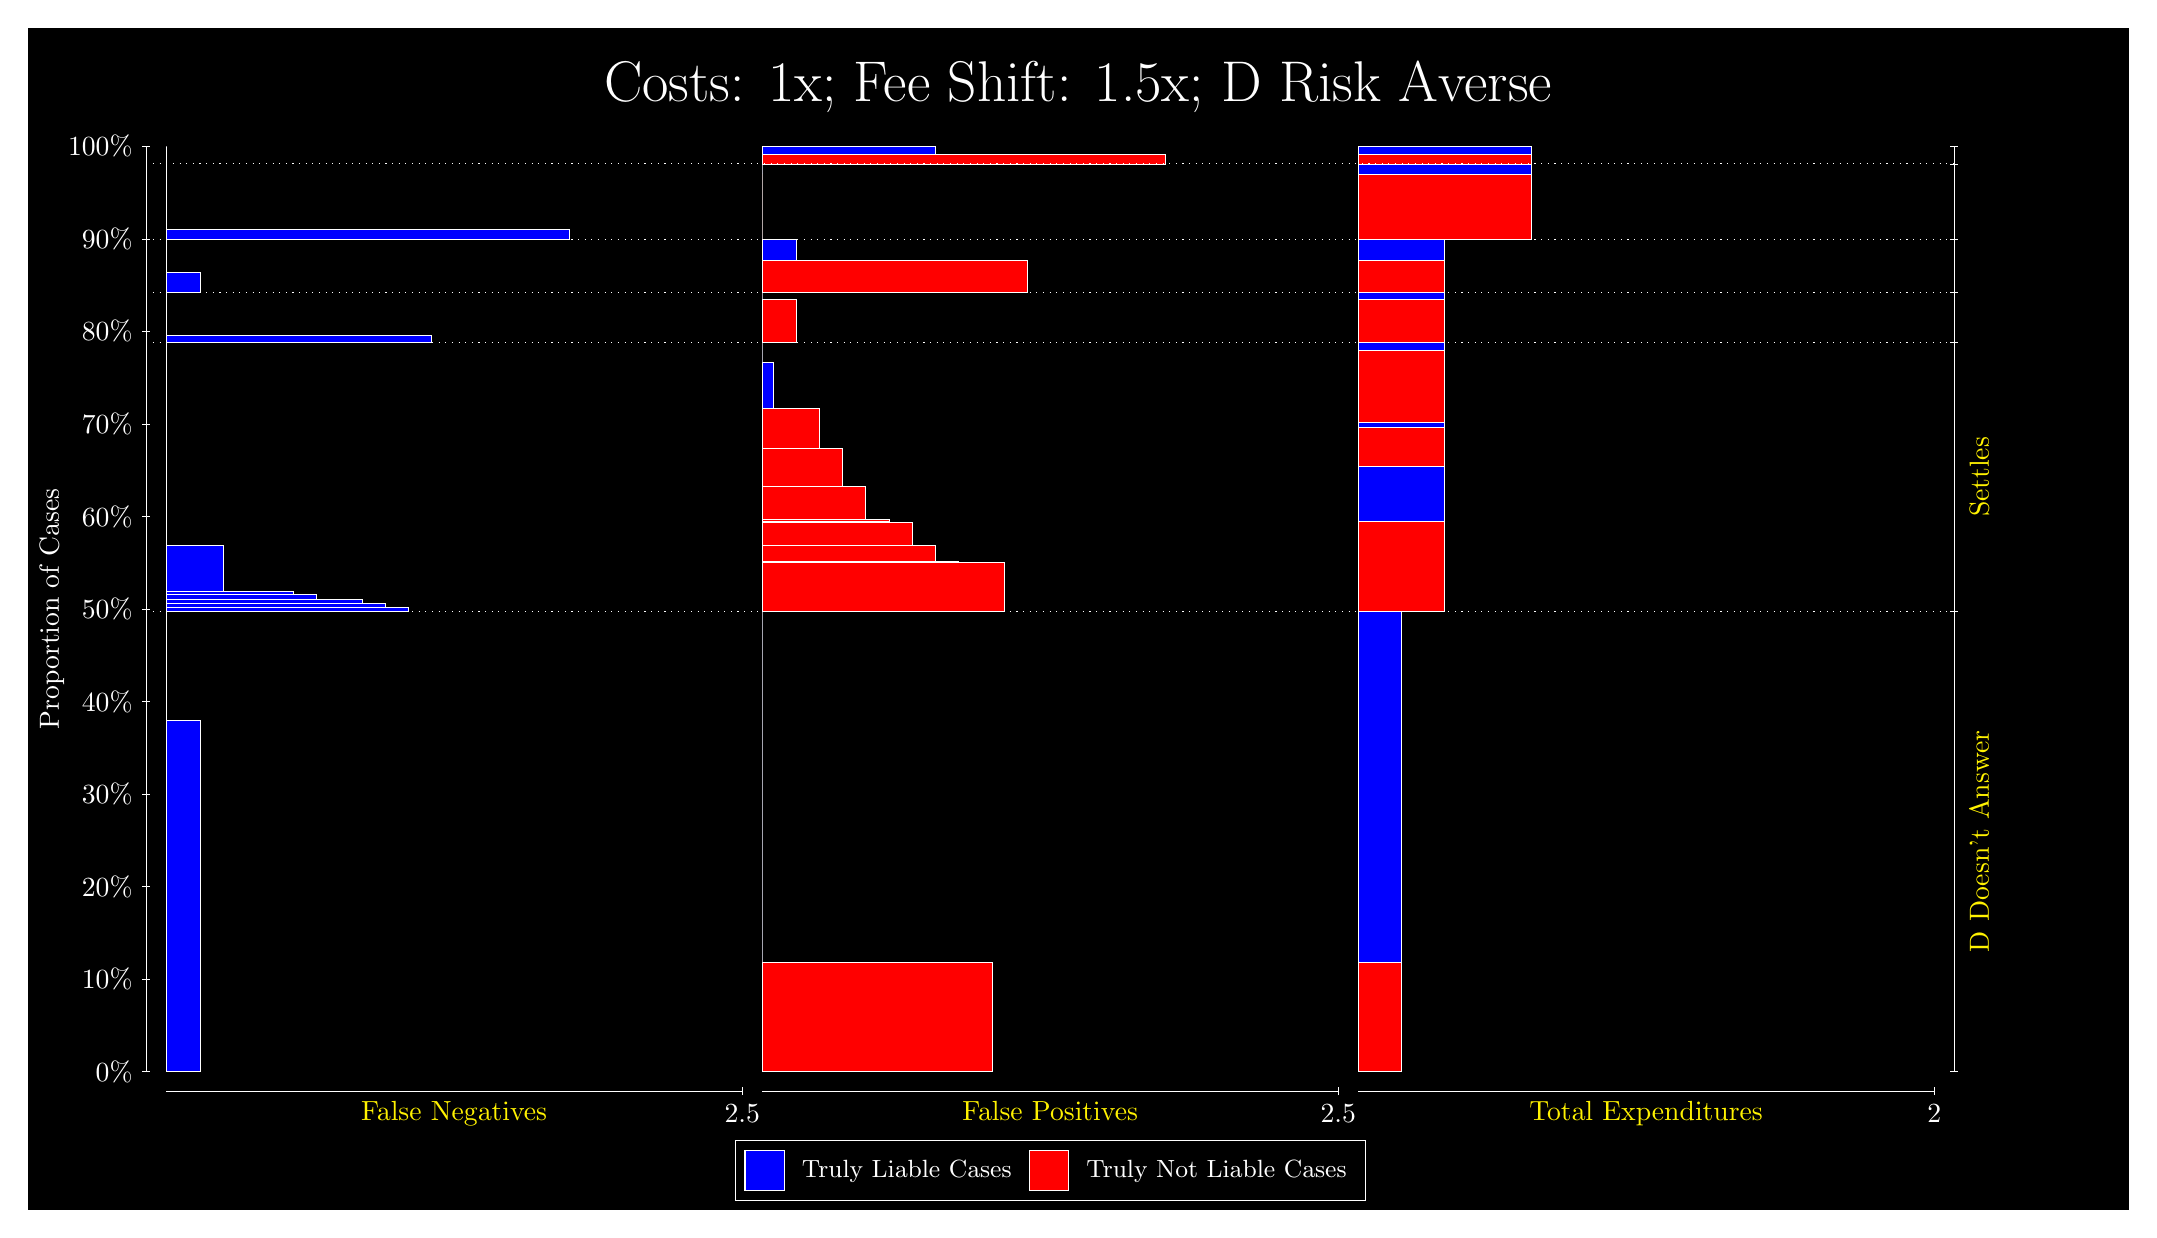
\begin{tikzpicture}
\draw[fill=black] (0,0) rectangle (26.667,15);
\draw[text=white] (0,13.5) rectangle (26.667,15) node[midway] {\huge Costs: 1x; Fee Shift: 1.5x; D Risk Averse};
\draw[white, very thin] (1.5,1.75) -- (1.5,13.5);
\node[rotate=90, text=white, anchor=center] at (0.3, 7.625) {Proportion of Cases};
\draw[white, very thin] (1.45,1.75) -- (1.55,1.75);
\node[text=white, anchor=east] at (1.45, 1.75) {0\%};
\draw[white, very thin] (1.45,2.925) -- (1.55,2.925);
\node[text=white, anchor=east] at (1.45, 2.925) {10\%};
\draw[white, very thin] (1.45,4.1) -- (1.55,4.1);
\node[text=white, anchor=east] at (1.45, 4.1) {20\%};
\draw[white, very thin] (1.45,5.275) -- (1.55,5.275);
\node[text=white, anchor=east] at (1.45, 5.275) {30\%};
\draw[white, very thin] (1.45,6.45) -- (1.55,6.45);
\node[text=white, anchor=east] at (1.45, 6.45) {40\%};
\draw[white, very thin] (1.45,7.625) -- (1.55,7.625);
\node[text=white, anchor=east] at (1.45, 7.625) {50\%};
\draw[white, very thin] (1.45,8.8) -- (1.55,8.8);
\node[text=white, anchor=east] at (1.45, 8.8) {60\%};
\draw[white, very thin] (1.45,9.975) -- (1.55,9.975);
\node[text=white, anchor=east] at (1.45, 9.975) {70\%};
\draw[white, very thin] (1.45,11.15) -- (1.55,11.15);
\node[text=white, anchor=east] at (1.45, 11.15) {80\%};
\draw[white, very thin] (1.45,12.325) -- (1.55,12.325);
\node[text=white, anchor=east] at (1.45, 12.325) {90\%};
\draw[white, very thin] (1.45,13.5) -- (1.55,13.5);
\node[text=white, anchor=east] at (1.45, 13.5) {100\%};

\draw[white, very thin] (24.457,1.75) -- (24.457,13.5);
\draw[white, very thin] (24.407,1.75) -- (24.507,1.75);
\node[anchor=west] at (24.407, 1.75) {};
\draw[white, very thin] (24.407,7.5971) -- (24.507,7.5971);
\node[anchor=west] at (24.407, 7.5971) {};
\draw[white, very thin] (24.407,11.007) -- (24.507,11.007);
\node[anchor=west] at (24.407, 11.007) {};
\draw[white, very thin] (24.407,11.643) -- (24.507,11.643);
\node[anchor=west] at (24.407, 11.643) {};
\draw[white, very thin] (24.407,12.32) -- (24.507,12.32);
\node[anchor=west] at (24.407, 12.32) {};
\draw[white, very thin] (24.407,13.278) -- (24.507,13.278);
\node[anchor=west] at (24.407, 13.278) {};
\draw[white, very thin] (24.407,13.5) -- (24.507,13.5);
\node[anchor=west] at (24.407, 13.5) {};

\draw[white, very thin, fill=blue] (1.75,1.75) rectangle (2.1891,6.2085);
\draw[white, very thin, fill=red] (1.75,6.2085) rectangle (1.75,7.5971);
\draw[white, very thin, fill=blue] (1.75,7.5971) rectangle (4.8239,7.6522);
\draw[white, very thin, fill=blue] (1.75,7.6522) rectangle (4.5312,7.7021);
\draw[white, very thin, fill=blue] (1.75,7.7021) rectangle (4.2384,7.7419);
\draw[white, very thin, fill=blue] (1.75,7.7419) rectangle (3.9457,7.7484);
\draw[white, very thin, fill=blue] (1.75,7.7484) rectangle (3.6529,7.8088);
\draw[white, very thin, fill=blue] (1.75,7.8088) rectangle (3.3602,7.8472);
\draw[white, very thin, fill=blue] (1.75,7.8472) rectangle (3.0674,7.8501);
\draw[white, very thin, fill=blue] (1.75,7.8501) rectangle (2.7746,7.8529);
\draw[white, very thin, fill=blue] (1.75,7.8529) rectangle (2.4819,8.4375);
\draw[white, very thin, fill=red] (1.75,8.4375) rectangle (1.75,11.007);
\draw[white, very thin, fill=blue] (1.75,11.007) rectangle (5.1167,11.096);
\draw[white, very thin, fill=red] (1.75,11.096) rectangle (1.75,11.643);
\draw[white, very thin, fill=blue] (1.75,11.643) rectangle (2.1891,11.905);
\draw[white, very thin, fill=red] (1.75,11.905) rectangle (1.75,12.32);
\draw[white, very thin, fill=blue] (1.75,12.32) rectangle (6.8732,12.449);
\draw[white, very thin, fill=red] (1.75,12.449) rectangle (1.75,13.278);
\draw[white, very thin, fill=red] (1.75,13.278) rectangle (1.75,13.403);
\draw[white, very thin, fill=blue] (1.75,13.403) rectangle (1.75,13.5);
\draw[white, very thin, fill=red] (9.3189,1.75) rectangle (12.246,3.1385);
\draw[white, very thin, fill=blue] (9.3189,3.1385) rectangle (9.3189,7.5971);
\draw[white, very thin, fill=red] (9.3189,7.5971) rectangle (12.393,8.2171);
\draw[white, very thin, fill=red] (9.3189,8.2171) rectangle (12.1,8.2209);
\draw[white, very thin, fill=red] (9.3189,8.2209) rectangle (11.807,8.2249);
\draw[white, very thin, fill=red] (9.3189,8.2249) rectangle (11.515,8.4332);
\draw[white, very thin, fill=red] (9.3189,8.4332) rectangle (11.222,8.7221);
\draw[white, very thin, fill=red] (9.3189,8.7221) rectangle (10.929,8.7395);
\draw[white, very thin, fill=red] (9.3189,8.7395) rectangle (10.929,8.7638);
\draw[white, very thin, fill=red] (9.3189,8.7638) rectangle (10.636,9.1773);
\draw[white, very thin, fill=red] (9.3189,9.1773) rectangle (10.344,9.661);
\draw[white, very thin, fill=red] (9.3189,9.661) rectangle (10.051,10.167);
\draw[white, very thin, fill=blue] (9.3189,10.167) rectangle (9.4652,10.752);
\draw[white, very thin, fill=blue] (9.3189,10.752) rectangle (9.3189,11.007);
\draw[white, very thin, fill=red] (9.3189,11.007) rectangle (9.758,11.555);
\draw[white, very thin, fill=blue] (9.3189,11.555) rectangle (9.3189,11.643);
\draw[white, very thin, fill=red] (9.3189,11.643) rectangle (12.686,12.058);
\draw[white, very thin, fill=blue] (9.3189,12.058) rectangle (9.758,12.32);
\draw[white, very thin, fill=red] (9.3189,12.32) rectangle (9.3189,13.149);
\draw[white, very thin, fill=blue] (9.3189,13.149) rectangle (9.3189,13.278);
\draw[white, very thin, fill=red] (9.3189,13.278) rectangle (14.442,13.403);
\draw[white, very thin, fill=blue] (9.3189,13.403) rectangle (11.515,13.5);
\draw[white, very thin, fill=red] (16.888,1.75) rectangle (17.437,3.1385);
\draw[white, very thin, fill=blue] (16.888,3.1385) rectangle (17.437,7.5971);
\draw[white, very thin, fill=red] (16.888,7.5971) rectangle (17.986,8.7395);
\draw[white, very thin, fill=blue] (16.888,8.7395) rectangle (17.986,9.4311);
\draw[white, very thin, fill=red] (16.888,9.4311) rectangle (17.986,9.9372);
\draw[white, very thin, fill=blue] (16.888,9.9372) rectangle (17.986,9.9924);
\draw[white, very thin, fill=red] (16.888,9.9924) rectangle (17.986,10.914);
\draw[white, very thin, fill=blue] (16.888,10.914) rectangle (17.986,11.007);
\draw[white, very thin, fill=red] (16.888,11.007) rectangle (17.986,11.555);
\draw[white, very thin, fill=blue] (16.888,11.555) rectangle (17.986,11.643);
\draw[white, very thin, fill=red] (16.888,11.643) rectangle (17.986,12.058);
\draw[white, very thin, fill=blue] (16.888,12.058) rectangle (17.986,12.32);
\draw[white, very thin, fill=red] (16.888,12.32) rectangle (19.083,13.149);
\draw[white, very thin, fill=blue] (16.888,13.149) rectangle (19.083,13.278);
\draw[white, very thin, fill=red] (16.888,13.278) rectangle (19.083,13.403);
\draw[white, very thin, fill=blue] (16.888,13.403) rectangle (19.083,13.5);
\draw[white, dotted] (1.5,7.5971) -- (24.457,7.5971);
\draw[white, dotted] (1.5,11.007) -- (24.457,11.007);
\draw[white, dotted] (1.5,11.643) -- (24.457,11.643);
\draw[white, dotted] (1.5,12.32) -- (24.457,12.32);
\draw[white, dotted] (1.5,13.278) -- (24.457,13.278);
\draw[white, very thin] (1.75,1.5) -- (9.0689,1.5);
\node[text=yellow, anchor=north] at (5.4094, 1.5) {False Negatives};
\draw[white, very thin] (9.0689,1.45) -- (9.0689,1.55);
\node[text=white, anchor=north] at (9.0689, 1.45) {2.5};

\draw[white, very thin] (9.3189,1.5) -- (16.638,1.5);
\node[text=yellow, anchor=north] at (12.978, 1.5) {False Positives};
\draw[white, very thin] (16.638,1.45) -- (16.638,1.55);
\node[text=white, anchor=north] at (16.638, 1.45) {2.5};

\draw[white, very thin] (16.888,1.5) -- (24.207,1.5);
\node[text=yellow, anchor=north] at (20.547, 1.5) {Total Expenditures};
\draw[white, very thin] (24.207,1.45) -- (24.207,1.55);
\node[text=white, anchor=north] at (24.207, 1.45) {2};

\node[text=yellow, centered, rotate=90] at (24.777, 4.6735) {D Doesn't Answer};
\node[text=yellow, centered, rotate=90] at (24.777, 9.3023) {Settles};





\draw (12.978300999999998,1.5) node[draw=none] (baseCoordinate) {};
\begin{scope}[align=center]
        \matrix[scale=0.5, draw=white, below=0.5cm of baseCoordinate, nodes={draw}, column sep=0.1cm]{
            \node[rectangle, draw, minimum width=0.5cm, minimum height=0.5cm, fill=blue] {}; &
            \node[draw=none, font=\small, text=white] (B) {Truly Liable Cases}; &
            \node[rectangle, draw, minimum width=0.5cm, minimum height=0.5cm, fill=red] {}; &
            \node[draw=none, font=\small, text=white] (B) {Truly Not Liable Cases}; \\
            };
\end{scope}

\end{tikzpicture}
\end{document}